
\chapter{结合静态程序分析的高效符号执行技术研究}
\label{chap-4}
%wb
符号执行作为一种典型的动态测试方法,在理论上能够有效遍历目标软件的
状态空间,从而深度挖掘软件中存在的漏洞。但对复杂
的源代码软件进行完整的符号执行测试是一个NP完全问题。因此,现有的测试方
法必须在完备性和有效性之间做权衡。%wb
导致符号执行路径空间爆炸的一个非常关键的因素是程序中的循环语句。在分析循环程序时,符号执行每一次进入循环体内部,都需要构造两条分支路径,分别对应了循环条件为真或假的情况。
总共的分支路径数目随着循环次数的增加呈指数级增加。
特别的,如果循环控制变量与输入相关,且没有对循环展开次数进行人为的限定,则循环将进行无限展开,甚至一个简单的循环将直接导致符号执行的路径爆炸问题。
目前试图缓解路径空间爆炸问题的方式是,
在符号执行的具体实现中,设计出好的路径遍历策略或者路径调度算法来提高符号执行的分析性能,
以便在有限的时间和内存消耗范围内达到最大的代码检测覆盖率。
在给定的遍历策略下,
通过限定每个循环的遍历次数来缓解该问题所产生的影响,
或者通过设置时间上限或者内存空间上限来缓解路径爆炸引起的分析工具崩溃的问题。
但是这些路径遍历策略或者调度算法都只是局部改进,很难从根本上解决这一问题。

本章提出了一种基于抽象解释静态分析的高效符号执行技术。给定待分析的源程序,首先解析出程序的控制流图。区别于其他符号执行技术,新技术通过静态程序分析方法,从程序的控制流图中计算出循环程序的不变式,然后对程序进行插桩用循环不变式代替循环,形成新的控制流图。在新的控制流图上进行符号执行,符号执行的路径将大大减少。

\section{问题描述}

考虑图\ref{fig-example1}中所示C程序片段,希望检测程序执行至第九行时,
是否存在输入$a$和$b$使得断言$assert(x \neq y)$不被满足。
由于变量$a$和$b$各自均有$2^{32}$个可能的取值,通过随机测试的方式检测程序是否存在错误是不可行的。
符号执行将输入变量的取值符号化,并在符号值上模拟程序的执行,遍历所有可能的程序路径。

\begin{figure}[h]
\begin{lstlisting}
void foobar(int a, int b){
  int x = 1, y = 0;
  if (a != 0) {
    y = 3+x;
	if (b == 0) {
	  x = 2 * (a+b);
	}
  }
  assert(x != y);
}
\end{lstlisting}
\caption{示例程序1}
\label{fig-example1}
\end{figure}

程序路径是程序的一个语句序列,包括一系列程序中顺序执行的代码片段,
代码片段之间的连接代表了分支语句导致的控制转移。
一个路径是可行的,是指至少存在一组具体的程序输入变量取值,
使得程序以该组取值作为输入,将沿着这条路径执行。反之,路径就是不可行的。
对于一条程序路径,路径条件是一个关于程序输入变量的符号值的约束。
一组输入值使得程序沿着这条路径执行当且仅当这组输入值满足这条路径的路径条件。

具体地,符号执行的计算过程通常可表示为三元组的形式:$(stmt, \sigma, \pi)$,其中,
$stmt$表示当前被分析的程序指令,例如赋值语句,条件语句或者函数调用;
$\sigma$表示程序路径中不同位置处变量的值,(可以是符号值,也可以是常量,或二者形成的函数),$\sigma$通常用函数映射表示;
$\pi$称为路径约束,是路径在各个分支执行点(位置)的分支条件(通常是一阶谓词及其布尔合成)的合取,
$\pi$的初始值为布尔常量$true$。

依据$stmt$的不同,符号执行采用不同的计算方式更新$\sigma$和$\pi$的取值:
\begin{enumerate}
\item 如果$stmt$是赋值语句$x = e$,其中表达式$e$可能是常数,变量或者函数应用,
	符号执行将更新$\sigma$中变量$x$的取值为$e$的符号值;
\item 如果$stmt$是条件语句$\text{if } e \text{ then } s_1 \text{ else } s_2$,
	符号执行将构造两条分支路径,分别对应了条件语句取值为真和假的两个情况,
	并更新两条分支路径的路径约束为: $\pi_{true} = \pi \wedge e$, 
	$\pi_{false} = \pi \wedge  \neg e$。
\end{enumerate}


\begin{figure}[h]
\centering
\begin{minipage}{0.3\textwidth}
%\begin{figure}
	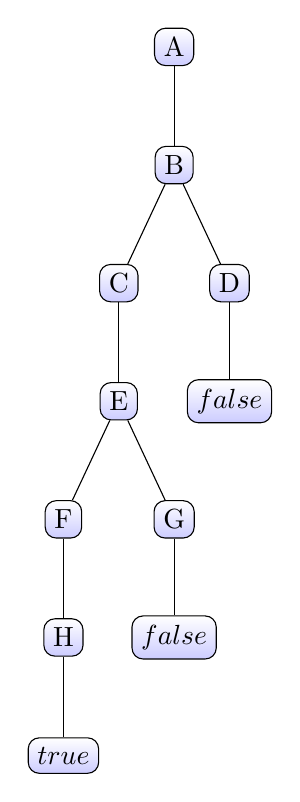
\begin{tikzpicture}[sibling distance=4em,
	every node/.style = {shape=rectangle, rounded corners, draw,
		top color=white, bottom color=blue!20}]]
	\node {A}
	child { node {B } 
		child { node { C }
			child { node { E }
				child {node {F}
					child {node {H}
						child {node {$true$}}
					}
				}
				child {node {G}
					child {node {$false$}}
				}
			}
		}
		child { node { D }
			child {node {$false$}
			}
		}
	};
	\end{tikzpicture}
%\end{figure}
\end{minipage}%
\begin{minipage}{0.7\textwidth}
\begin{tabular}{| c | c | c | c | }
	\hline
	节点 & $\sigma$ & $\pi$ & $stmt$ \\ 
	\hline		
	A & $ \{a = m, b = n\}$ & $ true$ & $x =1, y=0$ \\
	B & $\{a = m, b = n, x=1, y=0\}$ & $ true$ & $if(a\neq 0)$ \\
	C & $\{a = m, b = n, x=1, y=0\}$ &  $ m\neq 0$ & $y=3+x$ \\
	D & $\{a = m, b = n, x=1, y=0\}$ & $ m = 0$ & $assert(x\neq y)$ \\
	E & $\{a = m, b = n, x=1, y=4\}$ &  $ m\neq 0$ &  $if(b=0)$ \\
	F & $\{a = m, b = n, x=1, y=4\}$ & $ m \neq 0 \wedge n =0 $ & $x = 2*(a+b)$ \\
	G & $\{a = m, b = n, x=1, y=4\}$ & $ m \neq 0 \wedge n \neq 0 $ & $assert(x\neq y)$ \\
	H & $\{a = m, b = n, x=2(m+n), y=4\}$ & $ m \neq 0 \wedge n =0 $ & $assert(x\neq y)$ \\
	\hline  
\end{tabular}
\end{minipage}
\caption{示例程序1符号执行树及其计算过程}
\end{figure}


图\ref{fig-example1}中C程序代码的符号执行过程如下图所示,
左边部分表示了符号执行的执行树,右边的表格列出了执行树的每个节点中的数据信息。

从执行树中,可以看出路径$ABDEFH$表示了一条从程序初始入口到目标断言的执行,
该路径由指令序列$x=1,y=0;if(a\neq 0);y=3+x;if(b==0);x=2*(a+b);assert(x\neq y)$构成。
在断言位置,程序变量的符号取值为$\sigma = \{a = m, b = n, x=2(m+n), y=4\}$,
路径约束为$m \neq 0 \wedge n =0$, 其中,$m,n$为符号值。
那么,检测断言是否满足可以转化为检测逻辑公式
$x=2(m+n) \wedge y=4 \wedge m \neq 0 \wedge n =0 \wedge x == y$是否可满足。
一阶逻辑的可满足性可以通过约束求解器SMT求解。
通过约简,可以容易得到当$m = 2, n = 0$时,断言$assert(x\neq y)$不被满足。

从图\ref{fig-example1}中也可以看出,符号执行中,
每一个分支条件语句都可能会使当前的路径再分支出一条新的路径。
执行树的分支数(即程序路径数),随条件语句的数目的增加而增长,且增长关系是指数级的。
当分支数目变得巨大时,程序路径数目也将变得庞大而使得计算不可行,该问题称为路径爆炸问题。
%相对于上述符号执行技术,即所有变量都使用符号值约束,
%动态符号执行在分支语句时使用具体值的约束。
%因此,动态符号执行的在当前路径执行过程中不会产生新路径,
%只在执行结束后再去产生新路径,且一次只产生一条。
%但是,无论静态符号执行还是动态符号执行,都没法从根本上避免路径状态空间爆炸所造成的影响。

导致符号执行路径空间爆炸的另一个关键因素是程序中的循环语句,例如图\ref{fig-example2}中所示的while循环。
在分析这类循环程序时,符号执行每一次进入循环体内部,都需要构造两条分支路径,分别对应了循环条件为真或假的情况。总共的分支路径数目随着循环次数的增加呈指数级增加。特别的,如果循环控制变量输入相关,且没有对循环展开次数进行人为的限定,则循环将进行无限展开,一个简单的循环将直接导致符号执行的路径爆炸问题。因此本章提出了一种基于抽象解释静态分析的高效符号执行技术用于缓解由循环引起的路径爆炸问题。


\begin{figure}[h]
\begin{lstlisting}
void LoopExample(int x) {
  int i = 3, p = x;
  while(p > 0) {
    i = i + 4;
    p = p - 1;
	if (i >= 80)
	  assert(0); //target1
  }
  if(i>78)
  	assert(0);//target2
}
\end{lstlisting}
\caption{示例循环程序}
\label{fig-example2}
\end{figure}

\section{技术方案研究}
针对程序中循环语句可能导致的路径空间爆炸问题,
本章提出了一种基于抽象解释的高效符号执行技术。
该技术方案的框示意图如图\ref{fig-framework}所示。
给定待分析的源程序,首先解析出程序的控制流图。区别于其他符号执行技术,
新技术通过静态程序分析方法,从程序的控制流图中计算出循环程序的不变式,然后对程序进行插桩用循环不变式代替循环,形成新的控制流图。在新的控制流图上进行符号执行,符号执行的路径将大大减少。图\ref{fig-framework}的左下部分为原始程序的符号执行路径,假设循环$b \rightarrow c \rightarrow d \rightarrow b$的循环次数是$n$,则在符号执行时此循环将生成$2^{n}$条路径。经过静态分析后,$b \rightarrow c \rightarrow d \rightarrow b$代表的循环由$b^{'}$代替。在对修改之后的控制流图进行符号执行时,原本的$2^{n}$用一条路径代替。简言之,新技术旨在通过基于抽象解释的静态程序分析技术合成循环的约束,
并将该约束提供给符号执行引擎,减少符号执行路径。

\begin{figure}[h]
	\centering
	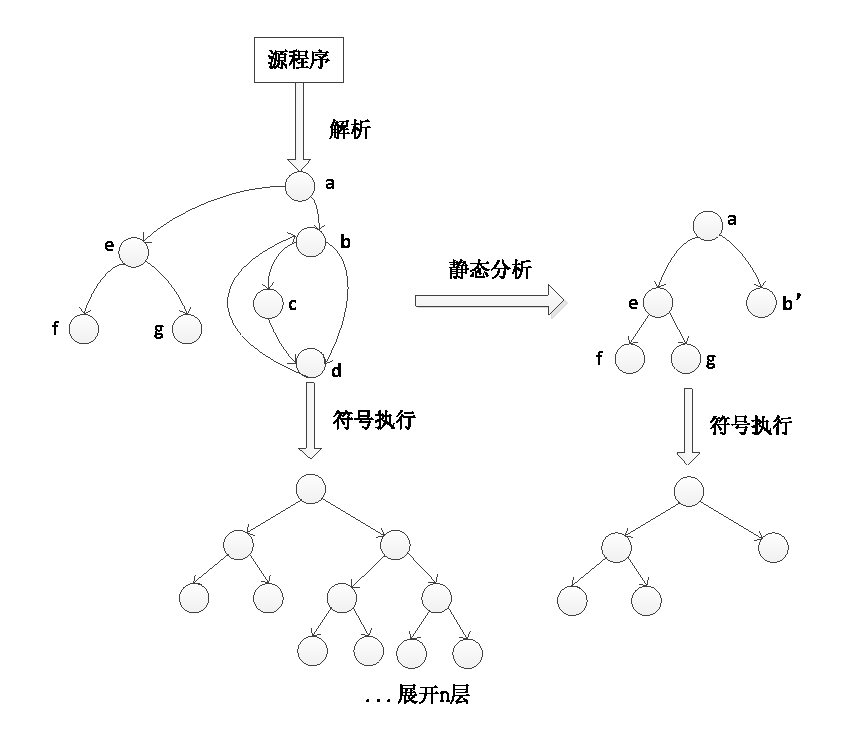
\includegraphics{figures/chap04/framework.pdf}
	\caption{基于抽象解释的符号执行技术框架}
	\label{fig-framework}
\end{figure}


%小节\ref{sec-absint}回顾了基于抽象解释的静态程序分析技术;
%小节\ref{sec-absint-symexe}详细论述本章提出的高效符号执行技术;
%小节\ref{sec-experiment}介绍了本章的实验设计与分析;
%小节\ref{sec-conclusion}对本章节进行总结。


\section{基于抽象解释的静态程序分析技术研究}
\label{sec-absint}

由于一般情况下,程序具体对象域上的不动点语义计算是不终止的,
基于抽象的静态程序分析技术通过构造一个抽象的对象域,将程序语义映射到抽象对象域上,
并构造程序的抽象不动点语义,作为对程序具体语义的逼近。
有效的抽象方法需要确保:(1)抽象域上的不动点语义计算是可行的;
(2)抽象语义是对具体语义的正确逼近。
抽象解释理论解决了如何快速计算程序不动点语义的问题,
在程序不动点语义计算的精确度和效率之间取得均衡,以低精确度的抽象计算换取较高的计算效率。
抽象解释为设计实用抽象技术,以及证明其的可靠性和正确性提供了理论工具。

%wq
抽象解释理论是Patrick Cousot及其夫人于1977年提出的静态程序分析理论。
基于抽象解释理论的静态程序分析技术的基本思想是,在保证抽象逼近可靠性的前提下,
对程序不动点语义计算过程的各个层次进行抽象逼近, 使得计算过程收敛或加速其收敛,
然后依据逼近计算的不动点语义验证程序需要满足的性质,
若验证过程中出现虚假反例, 则对抽象过程进行精化。
基于抽象解释理论的形式化验证的特点是可靠但不完备的。
如果分析结果表明抽象系统满足验证性质, 则抽象解释理论保证原程序也满足验证性质;
若验证结果表明抽象系统不满足验证性质,
则原系统可能满足验证性质(表明抽象过程中出现了不满足验证性质的虚假反例),
可能不满足验证性质(原系统存在不满足验证性质的真实反例), 需要更精细的抽象分析。
%wq copy



\subsection{抽象解释理论框架}

首先介绍抽象解释理论的数学基础。
直观上,程序语义的对象域是是程序运算的对象,包括了程序变量所有可能的取值集合。
数学上,通过一个偏序集合来刻画。

\begin{definition}
集合$<L, \subseteq>$称为偏序集合,
当且仅当,二元序关系$\subseteq$满足以下条件:
\begin{enumerate}
\item $\forall l \in L. (l,l)\in \subseteq$;
\item 如果 $(l,l_1)\in \subseteq \wedge (l_1, l')\in \subseteq$,
	那么$(l,l')\in \subseteq$;
\item 如果$(l,l')\in \subseteq$,$(l',l)\in \subseteq$,
	那么$l = l'$;
\end{enumerate}
\end{definition}


\begin{definition}
假设$<L, \subseteq>$是一个偏序集合,
$<L, \subseteq>$是一个完备格当且仅当:
$L$的任何一个子集均在$L$中存在最小上界和最大下界。
特别地,用$\sqcup$表示最小上界算子,用$\sqcap$表示最大下界算子,
用$\bot$表示最小元素,用$\top$表示最大元素。
完备格通常表示为$<L, \subseteq, \sqcup, \sqcap, \bot, \top>$.
\end{definition}


具体对象域与抽象对象域之间的映射的关系可以通过一对算子来刻画。
数学上,这对算子构成了一个Galois连接。


\begin{definition}
设$<P, \leq>$和$<Q, \subseteq>$是两个偏序集合,$\alpha:P \rightarrow Q$,
$\gamma: Q \rightarrow P$是两个映射,序偶$<\alpha, \gamma>$称为一个Galois连接当且仅当:
$\forall x\in P, \forall y\in Q. \alpha(x) \subseteq y$当且仅当$x\leq \gamma(y)$,
其中,映射$\alpha$称为抽象算子,$\gamma$称为具体算子。
\end{definition}

\begin{figure}[h]
\centering
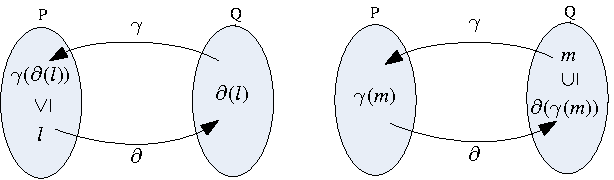
\includegraphics{figures/chap04/galois.pdf}
\caption{Galois连接示意图}
\label{fig-galois}
\end{figure}

由Galois连接的定义,容易得到如下关于抽象算子和具体算子的引理。

\begin{lemma}
序偶$<\alpha, \gamma>$是偏序集$<P, \leq>$和$<Q, \subseteq>$上的一个Galois连接, 则
\begin{enumerate}
\item $\forall x\in P. x \leq \gamma(\alpha(x))$;
\item $\forall y\in Q. \alpha(\gamma(y)) \subseteq y$;
\item $\alpha$和$\gamma$单调递增函数。
\end{enumerate}
\end{lemma}
	
\begin{proof}
$\forall x\in P. \alpha(x) \in Q$. 
由于$<Q, \subseteq>$是一个偏序集合,则$\alpha(x) \subseteq \alpha(x)$.
依据Galois连接的定义,得到$ x \leq \gamma(\alpha(x))$(将右边的$\alpha(x)$视为$y$)。
同理,$\forall y \in Q. \gamma(y) \in P$.
由于$<P, \leq>$是一个偏序集合,则$\gamma(y) \leq \gamma(y)$.
依据Galois连接的定义,得到$\alpha(\gamma(y)) \subseteq y$(将右边的$\gamma(y)$视为$x$)。\\
由于$\forall x\in P. x\leq \gamma(\alpha(x))$,以及偏序关系的传递性,
容易得知$ x\leq \gamma(\alpha(\gamma(\alpha(x))))$,
依据Galois连接的定义,进一步得到$\alpha(x)\subseteq \alpha(\gamma(\alpha(x)))$,
故$\alpha$算子是单调递增的。
同理可证$\gamma$的单调递增性。
\end{proof}


由于在程序具体对象域上计算语义最小不动点是不可行的,
基于抽象解释理论,可以通过抽象算子,将不动点计算映射到抽象对象域上,
并通过具体算子将抽象的计算结果映射到程序具体对象域上逼近实际的语义不动点。
假设程序$Prog$的最小不动点语义(即可达状态空间)为$LFP(Post_{Prog})$,
通过Galois连接$<\alpha, \gamma>$,定义程序的抽象后继算子
$AbsPost_{Prog} = \alpha \bullet Post \bullet \gamma$,
其中,符号$\bullet$表示函数合成,
那么程序的最小不动点语义可以用抽象$LFP(AbsPost_{Prog})$逼近。
Galois连接的性质保证了抽象不动点是对实际语义不动点的正确逼近。

在实际应用中,抽象域上的不动点计算也不一定终止。
程序不动点语义的计算过程不收敛是引起程序验证过程中状态空间爆炸的另一个原因。
假设$<L,\subseteq, \sqcup, \sqcap, \bot,\top>$是一个完备格,
程序的操作语义可以由完备格上的单调语义泛函$Post$来刻画,
理想情况下,$Post$算子是完备格$L$上的单调连续函数,
并且不动点计算$\bigcup_{i=0}\{Post^{i}\}$能够在有限次迭代计算后收敛。
然而,在实际情况下,不动点计算不一定在有限次迭代过程中收敛,
即便收敛,也不一定收敛到最小不动点。
在抽象解释的理论框架中,Widening算子可以给出一个不动点计算的上界逼近,
而Narrowing算子给出更加精细的上界逼近。

\begin{definition}[Widening算子]
假设$<L,\subseteq, \sqcup, \sqcap, \bot,\top>$是一个完备格,
算子$\nabla: L \rightarrow L$是一个Widening算子,当且仅当,
\begin{enumerate}
\item $\nabla$是一个上界算子;
\item 对于任意的递增链$(l_n)_n$,
递增链$(l_{n}^{\nabla})_n$收敛,其中,
$l_{n}^{\nabla} = l_0$,当$n=0$;
 $l_{n}^{\nabla} = l_{n-1}^{\nabla} \nabla l_n$,当$n>0$。
\end{enumerate}
\end{definition}

假设程序$Prog$的单调语义泛函$Post$定义在完备格
$<L,\subseteq, \sqcup, \sqcap, \bot,\top>$上,
并且算子$\nabla$是完备格上的一个Widening算子,
定义序列$Post_{n}^{\nabla}$为:

\begin{enumerate}
\item 若$n=0$,则$Post_{n}^{\nabla} = \bot$;
\item 若$n > 0$,并且
$Post(Post_{n-1}^{\nabla}) \subseteq Post_{n}^{\nabla}$,
则$Post_{n}^{\nabla} = Post_{n-1}^{\nabla}$;
\item 若$n > 0$,并且
$Post_{n}^{\nabla} \subseteq Post(Post_{n-1}^{\nabla})$,
则$Post_{n}^{\nabla} = Post(Post_{n-1}^{\nabla}) \nabla  Post_{n-1}^{\nabla}$。
\end{enumerate}

可以证明序列$Post_{n}^{\nabla}$是收敛的,
并且存在$m > 0$,使得$Post(Post_{m}^{\nabla}) \subseteq Post_{m}^{\nabla}$,
且$Post_{m}^{\nabla}$是最小不动点$LFP(Post)$的一个上界逼近。

\begin{definition}[Narrowing算子]
假设$<L,\subseteq, \sqcup, \sqcap, \bot,\top>$是一个完备格,
算子$\triangle: L \rightarrow L$是一个Narrowing算子,当且仅当,
\begin{enumerate}
\item $\forall l_1,l_2 \in L$,如果$l_2 \subseteq l_1$,
	则$l_2 (l_2\triangle l_1) \subseteq l_1$;
\item 对于任意的递降链$(l_n)_n$,
	递降链$(l_{n}^{\triangle})_n$收敛,其中,
	$l_{n}^{\triangle} = l_0$,当$n=0$;
	$l_{n}^{\triangle} = l_{n-1}^{\triangle} \triangle l_n$,当$n>0$。
\end{enumerate}
\end{definition}

假设算子$\triangle$是完备格上的一个Narrowing算子,
定义序列$Post_{n}^{\triangle}$为:

\begin{enumerate}
	\item 若$n=0$,则$Post_{n}^{\triangle} = Post_{n}^{\nabla}$;
	\item 若$n > 0$,
	则$Post_{n}^{\triangle} = Post_{n-1}^{\triangle} \triangle Post(Post_{n-1}^{\triangle})$。
\end{enumerate}

可以证明$LFP(Post) \subseteq Post(Post_{m}^{\nabla}) 
\subseteq  Post_{n}^{\triangle} \subseteq Post_{m}^{\nabla}$。
$Post_{m}^{\triangle}$同样是$LFP(Post)$的一个上界逼近,
并且是一个较$Post_{m}^{\nabla}$更加精确的上界逼近。


\begin{example}
	区间抽象域的思想是通过一个区间去逼近变量的取值集合。
	设$Z$是一个整数集合,如果$a=min(Z), b=max(Z)$,
	那么区间$[a,b]$是对$Z$的逼近。
	区间域的序关系$\subseteq$定义如下: $[a,b] \subseteq [c,d]$,
	当且仅当$a \geq c$,并且$b \leq d$,
	既是区间$[a,b]$包含在区间$[c,d]$中。
	域中的最大元素是$(-\infty, +\infty)$,最小元素是空集$\emptyset$。
	
	区间抽象域含有无穷多个元素,且含有无穷递增序列,
	因此需要扩展算子($widening$)进行近似计算。
	区间域的扩展算子定义如下:
	
	\begin{enumerate}
	\item 如果$m_2 < m_1$,并且$n_2 < n_1$,		
	则$[m_1, n_1] \nabla [m_2, n_2] = [\bot, n1]$;
	\item 如果$m_1 < m_2$,并且$n_1 < n_2$,
	则$[m_1, n_1] \nabla [m_2, n_2] = [m_1, \top]$;
	\item 如果$m_2 < m_1$,并且$n_1 < n_2$,
	则$[m_1, n_1] \nabla [m_2, n_2] = [\bot, \top]$;
	\item  如果$m_1 < m_2$,并且$n_2 < n_1$,
	则$[m_1, n_1] \nabla [m_2, n_2] = [m_1, n1]$。
	\end{enumerate}
\end{example}

除区间域外,常用的抽象域还包括了八边形域、多项式域。
区间域的表达能力较弱,只能够刻画单个程序变量的取值约束,但是计算复杂度最低。
多项式域的表达能力最强,可以刻画程序变量的相互关系,但是计算复杂度高。

\subsection{基于抽象解释的静态程序分析}

基于抽象解释理论的程序语义不动点计算过程的基本思想在算法\ref{algo-absint-analysis}所示。
算法以待分析的程序$Prog$作为输入,并计算程序变量在各个程序位置的不动点语义。
形式化地,用函数$\Sigma$表示程序的语义不动点,
该函数是一个从程序控制节点集合到一阶逻辑公式的映射,给定程序控制节点$l\in L$,
$\Sigma(l)$表示了在该节点位置,程序变量所有可能取值的约束条件。
该约束条件可能是一个取值区间,或者是一个线性不等式,具体形式取决于不动点计算采用的抽象域。


\begin{algorithm}[h]
\renewcommand{\algorithmicrequire}{\textbf{Input:}}
\renewcommand{\algorithmicensure}{\textbf{Output:}}
\caption{基于抽象解释的静态程序分析算法(AbstractStaticAnalysis)}
\label{algo-absint-analysis}
\begin{algorithmic}[1]
\REQUIRE 待分析程序源码$Prog$
\ENSURE 程序变量在各个位置的约束映射$\Sigma$
\STATE 创建程序$Prog$的控制流图$CFG=(L, E, l_0)$
\STATE 创建初始约束映射$\Sigma : L/\{l_0\} \rightarrow \{false\} \bigcup \{l_0\} \rightarrow \{true\}$
\STATE 创建工作列表$worklist$
\STATE $worklist \gets \{l_{0}\}$
\WHILE{$worklist \neq \emptyset$}
	\STATE $l \gets $ pop($worklist$)
	\STATE $\sigma \gets \Sigma(l)$
	\IF{$l \neq l_0$}
		\STATE $\Gamma_I \gets $ InEdges($l$)
		\STATE $\sigma_{new} \gets \sigma$
		\FOR{$\gamma \in \Gamma_I$}
			\STATE $\gamma \gets (l',stmt,l)$
			\STATE $\sigma' \gets \Sigma(l')$
			\STATE $\sigma'' \gets post(\sigma', stmt)$
			\STATE $\sigma_{new} \gets \sqcup(\sigma, \sigma'')$
		\ENDFOR
		\IF{$\sigma_{new} \neq \sigma$}
			\STATE $\Sigma(l) \gets \sigma_{new}$
			\STATE $\Gamma \gets $ OutEdges($l$)
			\FOR{$\gamma \in \Gamma$}
				\STATE $\gamma \gets (l, stmt, l')$
				\STATE push($l'$, $worklist$)
			\ENDFOR
		\ENDIF
	\ELSE
		\STATE $\Gamma \gets $ OutEdges($l$)
		\FOR{$\gamma \in \Gamma$}
			\STATE $\gamma \gets (l, stmt, l')$
			\STATE push($l'$, $worklist$)
		\ENDFOR
	\ENDIF
\ENDWHILE
\end{algorithmic}
\end{algorithm}

算法首先构建程序的控制流图$CFG=(L, E, l_0)$,并对函数$\Sigma$进行初始化。
初始条件下,程序入口位置的约束为布尔常量$true$,其他位置的约束为常量$false$。
算法采用典型的工作列表设计模式,工作列表中存放待分析的程序节点。
算法每一次从工作列表中取出一个节点进行分析,并依据分析结果将该节点的后继节点放入列表中,
直至所有节点的分析完成,即工作列表为空。
初始条件下,工作列表仅含有程序的初始入口节点$l_0$。

对于程序的每个控制节点$l$,如果是初始节点,那么算法直接将其后继节点加入工作列表;
如果不是初始节点,算法将进行进一步的分析。
具体地,算法首先获取该节点$l$的所有前继语句$\Gamma_{I}$,
对每个语句$(l',stmt,l)\in \Gamma_{I}$,及其前继节点$l'$的约束$\sigma'$,
算法应用Post后继算子计算相对于语句$stmt$的后继约束条件$\sigma''$,
并应用抽象域中的上界算子$\sqcup$,得到当前节点$l$处的新的约束值$\sigma_{new} = 
\sqcup(\sigma,\sigma'')$。
上述计算$post(\sigma', stmt)$,$\sqcup(\sigma,\sigma'')$均在给定的抽象域上完成,
具体计算规则由抽象解释理论的抽象域给出。

随后,算法判断位置$l$的新约束$\sigma_{new}$是否与当前约束$\sigma$等价。
如果不等价,则更新该位置的约束为$\sigma_{new}$,
并将位置$l$的所有后继节点加入工作列表;
如果相同,说明该位置的约束已经包括了程序变量的所有可能取值。
当在每个位置的约束均覆盖了程序变量在该位置的所有可能取值时,算法终止。
抽象解释理论确保了算法的终止性。


本方法采用基于抽象解释理论的静态程序分析技术计算程序变量的约束关系,
例约束$x-p = (i-3)/4$,并使用该约束辅助符号执行。
基于多边形抽象域的静态分析技术可以计算上述形式的约束。

\section{结合静态程序分析的高效符号执行算法}
\label{sec-absint-symexe}

程序中的循环语句是导致符号执行路径爆炸问题的主要因素之一。
缓解该问题的解决方法主要包括了:
1:对循环体做有限次展开,以损失分析的完备性换取计算的可行性;
2:采用特殊的导向策略引导符号执行的路径遍历,
 避免对循环体做无限次展开;
3:基于循环摘要对循环语句进行抽象,该抽象是对循环体行为的刻画。
 对循环程序的分析可以转换为对循环摘要的分析。
本章提出了一种基于抽象解释的循环程序符号执行技术。
为提高对循环程序的分析效率,提出采用抽象解释技术计算出循环程序的语义逼近,
并用该抽象语义辅助符号执行技术。


\subsection{核心技术思想}

首先通过实例来解释本方法的技术方案。
考虑图\ref{fig-example2}所示循环程序片段, 为了检测程序是否能够执行至第七行,
符号执行进行路径搜索的同时,需要对while循环进行展开,展开次数与函数的输入参数$x$以及变量$i$相关。
理论上,对于该程序片段,符号执行需要对循环进行20次展开,那么就需要遍历$2^{20}$个程序路径。
图\ref{fig-tree2}和图\ref{fig-compute2}展示了对循环进行2次展开的符号执行过程。

\begin{figure}[h]
	\centering
		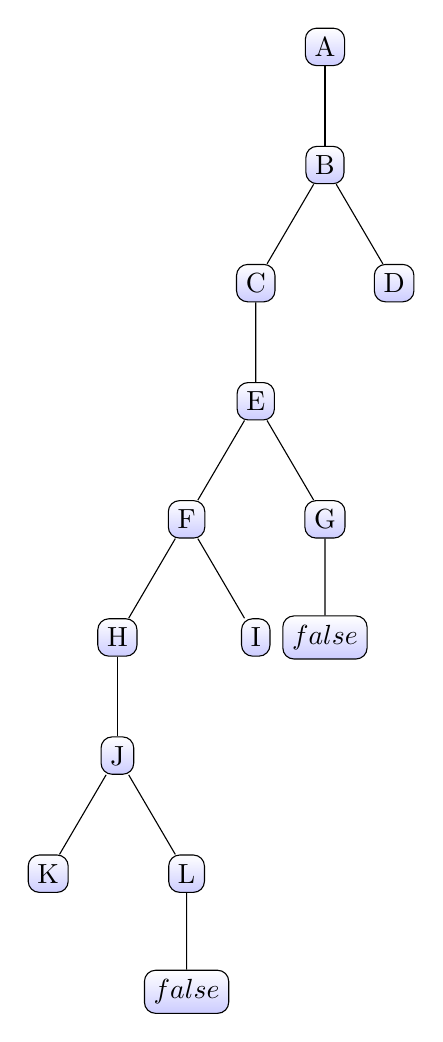
\begin{tikzpicture}[sibling distance=5em,
		every node/.style = {shape=rectangle, rounded corners, draw,
			top color=white, bottom color=blue!20}]]
		\node {A}
		child { node {B } 
			child { node { C }
				child { node { E }
					child {node {F}
						child {node {H}
							child {node {J}
								child {node {K}}
								child {node {L}
									child {node {$false$}}
								}
							}
						}
						child {node {I}}
					}
					child {node {G}
						child {node {$false$}}
					}
				}
			}
			child { node { D }}
		};
		\end{tikzpicture}
		\caption{示例程序2符号执行树}
		\label{fig-tree2}
\end{figure}

\begin{figure}[h]
		\begin{tabular}{| c | c | c | c | }
			\hline
			节点 & $\sigma$ & $\pi$ & $stmt$ \\ 
			\hline		
			A & $ \{x = m\}$ & $ true$ & $i=3, p=x$ \\
			B & $\{x = m, i=3, p=m\}$ & $ true$ & $while(p > 0)$ \\
			C & $\{x = m, i=3, p=m\}$ &  $ m > 0$ & $i=i+4;p=p-1$ \\
			D & $\{x = m, i=3, p=m\}$ & $ m \leq 0$ & $skip$ \\
			E & $\{x = m, i=7, p=m-1\}$ &  $ m> 0$ &  $if(i\geq 80)$ \\
			F & $\{x = m, i=7, p=m-1\}$ & $ m > 0 \wedge i < 80 $ & $while(p > 0)$ \\
			G & $\{x = m, i=7, p=m-1\}$ & $ m > 0 \wedge i \geq 80 $ & $abort()$ \\
			H & $\{x = m, i=7, p=m-1\}$ & $ m > 0 \wedge i < 80 \wedge m-1>0$ & $i=i+4;p=p-1$ \\
			I & $\{x = m, i=7, p=m-1\}$ & $ m > 0 \wedge i < 80 \wedge m-1 \leq 0$ & $skip$ \\
			J & $\{x = m, i=11, p=m-2\}$ & $ m > 0 \wedge i < 80 \wedge m-1>0$ & $if(i\geq 80)$ \\
			K & $\{x = m, i=11, p=m-2\}$ & $ m > 0 \wedge i < 80 \wedge m-1>0$ & $while(p>0)$ \\
			L & $\{x = m, i=11, p=m-2\}$ & $ m > 0 \wedge i \geq 80 \wedge m-1>0$ & $abort()$ \\
			\hline  
		\end{tabular}
	\caption{示例程序2符号执行计算过程}
	\label{fig-compute2}
\end{figure}

\begin{enumerate}
\item 符号执行树中,程序路径$ABCEG$表示了一条从初始入口到目标指令的执行路径。
该路径通过对循环进行一次展开得到,其对应的指令序列为
$i=3,p=x;while(p>0);i=i+4;p=p-1;if(i\geq 80);abort();$,
在目标指令位置,程序变量的符号取值为$x=m;i=7;p=m-1$,路径约束为$m>0\wedge i\geq 80$。
显然,当前变量$i$的取值不满足路径约束,所以该执行路径是不可行的。
\item 类似地,通过对循环进行两次展开,得到程序路径$ABCEFHJL$,其对应的指令序列为
$i=3,p=x;while(p>0);i=i+4;p=p-1;if(i < 80);while(p>0);i=i+4;p=p-1;if(i\geq 80);abort()$,
在目标指令位置,程序变量的符号取值为$x=m;i=11;p=m-2$,路径约束为$m>0\wedge i\geq 80 \wedge m-1>0$。
当前变量$i$的取值同样不满足路径约束,所以该执行路径是不可行的。
\item 以此类推,对循环进行第20次展示后,得到的程序变量符号约束为$x=m;i=83;p=m-20$,
路径约束为$i\geq 80 \wedge m-19>0$。
此时,变量$i$的取值满足路径约束,该执行路径是可行的,相应的输入变量的约束条件为$x>19$。
当目标指令所在的分支条件,即$i\geq 80$,发生改变,如$i\geq 100$,
那么循环的展开次数则变为$100$,此时符号执行树的分支数目增长为$2^{100}$。
由此可知,符号执行在分析此类循环程序时,即便程序规模很小,也难以在合适的时间内给出分析结果。
\end{enumerate}

进一步分析可知,为了快速高效地找到触发程序第一个目标$assert$指令的输入值,
关键是需要找到变量$p$和$i$的关系:$x-p = (i-3)/4$。
假设我们通过特定的程序分析技术得到了上述关系,那么在运行符号执行时,
例如当符号执行遍历路径$ABCEG$时,我们不使用当前路径的变量取值$x=m;i=7;p=m-1$,
而使用约束$x-p = (i-3)/4$去判定是否存在输入使得路径约束被满足。
由于约束$x-p = (i-3)/4 \wedge i\geq 80 \wedge p \geq 0$是可满足的,
得到输入变量的约束为$x>19$。

本质上,约束$x-p = (i-3)/4$刻画了程序变量在目标指令位置的所有可能取值。
例如,当程序通过路径$ABCEG$到达目标指令位置时,变量的取值为$x=m;i=7;p=m-1$,
显然,$x-p = (i-3)/4$。
当程序通过路径$ABCEFHJL$到达目标指令位置时,变量的取值为$x=m;i=11;p=m-2$,
同样满足上述约束。
在程序分析领域,约束$x-p = (i-3)/4$通常称为程序的循环不变式。


\subsection{高效符号执行算法}

该技术的核心思想如算法\ref{algo-absint-symexe}所示。大体上,算法分为两部分:静态分析部分和动态符号执行部分。算法接收待验证程序源码$Prog$作为输入,并初始化抽象执行树tree、工作列表以及程序语义不动点。抽象执行树的节点代表了程序的抽象状态,树的边表示程序的执行路径。
每个节点$\eta$包括了三部分信息:程序的指令位置$loc$,程序变量的符号取值$\sigma$和程序路径在当前位置的路径约束$\pi$。算法维护一个工作列表,里面的元素是待遍历的树节点,即程序状态。算法在进行符号执行式,逐次从工作列表中取出一个节点$\eta$进行分析,直至工作列表为空。
%依据节点的不同类型,算法进行相应的计算。程序的语义不动点是一个$<loc,constraints>$的二元组,$loc$表示的是程序指令位置,$constraints$表示$loc$位置上的约束。
结合静态程序分析的高效符号执行算法算法\ref{algo-absint-symexe}可分为以下过程。

%(1)对于程序$Prog$中的每个循环运行基于抽象解释的静态程序分析算法生成程序在各个位置的不动点(第6行),然后将不动点以注释的形式写入程序中。

%\begin{enumerate}
%\item 调用前向分析算法$ForwardAnalysis$对程序进行静态分析,生成程序语义不动点;
%
%\item 判断程序$Prog$中是否包含循环,若包含循环则获取循环的位置$locs$;
%
%\item 对于每一个循环的位置获取由静态分析的出来的约束集$constraints$;
%
%\item 对程序进行插桩,将循环替换为上一步的出来的约束;
%
%\item 对插桩后的程序进行符号执行。首先判断该节点是否代表了一个错误状态。
%如果是错误状态,那么就构造程序变量的符号取值$\sigma$和当前位置的路径约束$\pi$的合取$\sigma \wedge \pi$,
%并判断该合取是否可满足。如果可满足,说明该错误状态是可达的,并且公式$\sigma \wedge \pi$的可满足模型给出了
%导致程序执行至该错误状态的输入变量的取值。算法调用函数$BuildCEX$构造反例,该函数从当前节点$\eta$回溯至执行树的根节点。
%\item 如果该节点表示了一个程序的循环,即存在一个前继节点$\eta' = (loc', \sigma', \pi')$,使得$loc' = loc$,
%那么算法调用前向分析算法$ForwardAnalysis$对程序进行静态分析。
%\end{enumerate}

%程序的预处理,循环内部的所有的函数调用都进行内联,因为抽象解释工具不能处理函数调用的情况。

(1)对于程序$Prog$中的每个循环运行基于抽象解释的静态程序分析算法生成程序在各个位置的不动点(第3行),然后将不动点以注释的形式写入程序中(第4行),其中不动点是由各个变量的不变式组成。下面以图\ref{fig-example2}中的循环程序为例,阐述生成不变式的过程。首先在循环中加入一个初始值为0的计数变量counter,用于记录循环的展开次数。加入$counter$的目的是表达程序变量和循环展开次数的关系。为了在每个程序点产生不变式,本章在多面体抽象域\upcite{chen_interval_2009}中运行前向抽象解释算法进行静态分析。多面体抽象域是一个完全的数值关系域,可以用来表达任意的线性等式和不等式。多面体抽象域比数值域\upcite{chen_interval_2009}、五边形域\upcite{logozzo_pentagons:_2008}以及八边形域\upcite{mine_octagon_2006}表达能力更强,同时耗费的资源也更多。
如图\ref{fig-example3}第4行所示;此不变式表示要到达当前程序点变量$x$需要满足的约束条件。插入不动点的位置有三类:循环的入口处,分支语句处以及循环结束处,分别对应图\ref{fig-example3}的第4-5行、第9行以及第12-13行。

(2)在进行符号执行之前,需要通过插桩的方式插入特殊指令(第6行),使得在符号执行时能够辨别需要处理的循环对象。在每个循环的开始处插入"LSEntry"表示循环处理开始,如图\ref{fig-example3}的第3行;在循环的结束处插入“LSEnd”表示循环处理结束,如图\ref{fig-example3}的第15行。

\begin{figure}[h]
\begin{lstlisting}
void LoopExample(int x) {
  int i = 3, p = x;
  LSEntry;
  while(p > 0) {
  /* i = 4 * counter + 3, counter >= 0, counter <= 19,
   x = counter + p, p > 0 */
    i = i + 4;
    p = p - 1;
	if (i >= 80)
	/* i = 4 * counter + 3, counter = 20, x = counter + p, p > 0*/
	  assert(0); //target1
  }
  /* i = 4 * counter + 3, x = counter + p, counter >= 0, 
   counter <= 19, p < 0*/
   LSEnd;
   if(i>78)
     assert(0);//target2
}
\end{lstlisting}
\caption{注释后的循环实例程序}
\label{fig-example3}
\end{figure}

(3)动态符号执行的过程中会逐条读取指令,根据指令类型的不同执行不同的操作(第8-21行)。其中第9-15行为正常的符号执行过程。从$worklist$中取出一个$\eta$,判断当前位置是否存在错误(第10行),如果存在则调用约束求解器求解测试用例(第13行),然后返回测试用例。本章对符号执行的修改体现在对新添指令“LSEntry”和“LSEnd”的处理上(第17行)。动态符号执行最主要的三个操作是约束累积、更新内存(包括符号内存和具体内存)以及约束求解。图\ref{符号执行变换后的程序}是符号执行变换后程序的示意过程。以图\ref{fig-example3}中的程序为例,符号执行时将x符号化。当符号执行读取本章自定义的标识指令“LSEntry”时,则会根据抽象解释产生的注释做相应的操作。首先,新建表示循环展开次数的变量counter。然后,若目标区域包含在循环内部,则从注释/* i = 4 * counter + 3, counter = 20, x = counter + p, p > 0*/提取等式进行具体和符号内存更新,具体内存的更新为i=83,counter=20,符号内存的更新为x=20+p;提取不等式p>0更新符号约束
,进而约束求解求得满足约束的测试用例,此例中只要x>=20都能满足约束条件。若目标区域在循环外部,例如图\ref{fig-example3}的第17行,则从注释/* i = 4 * counter + 3, x = counter + p, counter >= 0, 
   counter <= 19, p < 0*/提取等式counter=x-p,i=4*counter+3更新内存,提取不等式counter>=0累积约束,返回到自定义标识指令“LSEnd”继续后面程序的符号执行。例如,在符号执行到图\ref{符号执行变换后的程序}第16行时,将i>78加入到约束并对约束求解,解得x=19就是到达第17行assert语句的输入。利用抽象解释产生的不变式,将图\ref{符号执行变换后的程序}的while循环变换成一个分支语句,一个指向循环中的目标区域,一个指向循环后的程序点;若目标区域不在循环内部,则将while循环变换成一个顺序语句。如此则能大大减少符号执行中因循环引起的执行状态。
%扩展的符号执行语义

\begin{figure}[htb]
\begin{center}
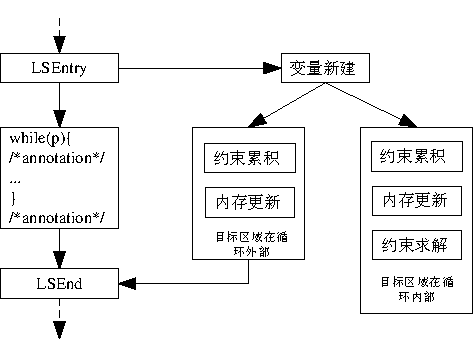
\includegraphics[scale=1.4]{chap04/符号执行变换后的程序}
\end{center}
\caption{符号执行变换后的程序}
\label{符号执行变换后的程序}
\end{figure}

%\begin{table}[ht]
%\begin{center}
%\caption{符号执行扩展语义} \label{符号执行扩展语义}
%\begin{small}
%\begin{tabular}{|c|c|c|}
%\hline 
%指令类型 & 指令示例 & 符号执行动作\tabularnewline
%\hline 
%Assign & x=y & Assign(x=y)\tabularnewline
%\hline 
%Exit & assert(0);abort();exit(); & solve();terminate();\tabularnewline
%\hline 
%Branch & if(x==5)\{\} & fork();addConstraints(x==5);\tabularnewline
%\hline 
%... &  & \tabularnewline
%\hline 
%LS & /{*} x = counter + p, counter >= 0, & Assign(x = counter + p);Assign(counter = (i-3)/4);\\ 
%   & counter <= 19, counter = (i-3)/4
%{*}/ & addConstraints(counter>= 0);counter <= 19
%\tabularnewline
%\hline 
%\end{tabular}
%\end{small}
%\end{center}
%\end{table}

\begin{algorithm}[h]
\renewcommand{\algorithmicrequire}{\textbf{Input:}}
\renewcommand{\algorithmicensure}{\textbf{Output:}}
\caption{基于静态程序分析的高效符号执行算法}
\label{algo-absint-symexe}
\begin{algorithmic}[1]
\REQUIRE 待分析程序$prog$
\ENSURE 程序bug,或者运行超时
%\STATE 初始化抽象执行树$tree$
%及其根节点$\eta_{root}$
%\STATE 初始化工作列表$worklist$
\STATE 初始化程序语义不动点 $fixpoint$
%\STATE $worklist \gets \{\eta_{root}\}$
\FOR{$loop$ in $prog$}
	\STATE $fixpoint$ = forwardAnalysis($loop$)
	\STATE annotate($fixpoint$)
\ENDFOR
\STATE $prog^{'}$ = instrument(prog)
\STATE $worklist$ = initilize($prog^{'}$)
%\STATE $fixpoint$ = forwardAnalysis(prog)
%\IF{ContainsLoop($prog$)}
%\STATE $locs$ = obtainLoopLoc($prog$)

%\ENDFOR
%\ENDIF
\WHILE{$worklist \neq \emptyset$}
	\STATE $\eta \gets $ pop($worklist$)
	\IF{IsError($\eta$)}
		\STATE $\eta = (loc, \sigma, \pi)$
		\IF{$\sigma \wedge \pi$ is SAT}
			\STATE $\mathit{cex}$ $\gets$ BuildCEX($\eta$)
			\RETURN $\mathit{cex}$
		\ENDIF
	
	\ELSE
		\STATE $\Gamma \gets $ ExtActions($\eta$)
		\STATE Successors($\eta$, $\Gamma$)
		\STATE add successors of $\eta$ into $worklist$
	\ENDIF
\ENDWHILE
\end{algorithmic}
\end{algorithm}


%\begin{theorem}
%给定待分析程序$prog$,假设$prog$中存在一个不安全状态$error$,
%则算法\ref{algo-absint-symexe}能够检测该程序是不安全的,
%并输入一条从程序初始入口到该不安全状态的执行路径。
%\end{theorem}
%
%\begin{proof}
%TODO
%\end{proof}



\section{实验与分析}
\label{sec-experiment}

\subsection{实验设计}

(1)实验目的

本实验的目的是在标准测试程序上验证结合静态程序分析的高效符号执行技术的有效性。验证本章方法相对于其他方法在挖掘漏洞上的效率;验证本章方法在漏洞挖掘数量上的优越性。

(2)实验环境

本节基于C语言编译器Clang\upcite{noauthor_clang_nodate}结合KLEE实现了本章提出的高效符号执行技术(Fast Symbolic Execution,FastSE)。在实验中,本节选取公开的测试程序源码作为测试集与符号执行工具KLEE进行对比。本实验的测试集取自2017年软件验证国际竞赛
\footnote{\url{https://sv-comp.sosy-lab.org/2017/}}
的测试用例库。测试集总共有100个测试程序。每个测试程序中均含有一条assert语句,并且均存在一组输入,使得程序运行至该语句时,该语句的取值为假。100个测试程序中有68个程序包含循环,其中15个包含嵌套循环。实验的采用的硬件环境是Inter Xeon CPU E3-1231 v3 @ 3.40GHz,16G RAM。本实验设置的符号执行停机时间是20分钟,设置的内存限制是12GB。为了保证
实验参数的一致性,对每一个测试程序设置的符号执行参数都是相同的。为了进行多方位的对比,除了原始的KLEE符号执行工具,本实验还将循环定长展开的KLEE也加入了实验。循环定长展开的KLEE在本实验中称为KLEE-Fix,定长展开的次数设定为10。

(3)实验过程

实验过程如图\ref{experiment_procedure}所示。对与每一个C源程序,首先,将其编译成LLVM IR;其次,在LLVM IR上做静态分析并将结果插桩到程序中;再次,在插桩后的程序上根据设计的特殊指令进行高效符号执行;最后,检查是否在未超时的情况下发现程序错误,从而生成测试用例。

\begin{figure}[h]
	\centering
	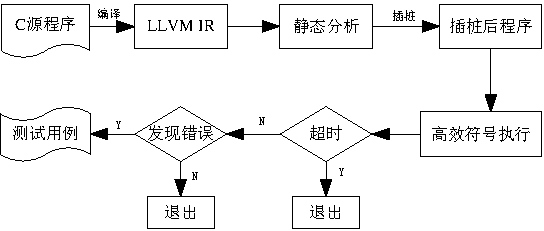
\includegraphics[scale=1.4]{chap04/结合静态程序分析的高效符号执行技术实验过程}
	\caption{结合静态程序分析的高效符号执行技术实验过程}
	\label{experiment_procedure}
\end{figure}

\subsection{结果分析}
表\ref{FastSE_KLEE-Fix与KLEE的发现错误数量以及总时间耗费对比}为FastSE、KLEE-Fix与KLEE在测试实例时的超过时间限制的实例数量、发现错误的实例数量以及总测试时间。从表\ref{FastSE_KLEE-Fix与KLEE的发现错误数量以及总时间耗费对比}可以看出,FastSE在三个方面都相对于KLEE和KLEE-Fast都具有优势,分别比KLEE-Fix和KLEE多检测了6和14个错误实例。从超过时间限制的实例数量可以看出,KLEE在符号执行有循环的传程序时会耗费大量的时间。如果将循环进行定长展开,符号执行时间大大减少的同时也会发现更多的错误。

\begin{table}[ht]
\begin{center}
\caption{FastSE、KLEE-Fix与KLEE的错误发现数量以及总时间耗费对比}
\label{FastSE_KLEE-Fix与KLEE的发现错误数量以及总时间耗费对比}
\begin{small}
\begin{tabular}{|l|l|l|l|}
\hline
{\bf } & {\bf Timeout数量} & {\bf 检测错误实例数量} & {\bf 总测试时间} \\
\hline
KLEE & 57 & 43 & 22小时17分12秒 \\
KLEE-Fix & 19 & 51 & 14小时13分34秒\\
FastSE & 11 & 57 & 12小时31分55秒\\
\hline
\end{tabular}
\end{small}
\end{center}
\end{table}

表\ref{FastSE_KLEE-Fix与KLEE发现错误数量交叉对比}是FastSE、KLEE-Fix与KLEE发现错误数量的交叉对比。“>”操作符表示前者发现错误而后者未发现错误的实例数量,例如FastSE > KLEE-Fix表示FastSE发现了错误而KLEE-Fix未发现的实例总数。从表\ref{FastSE_KLEE-Fix与KLEE发现错误数量交叉对比}可以看出三种方法发现的错误实例互有交叉而又互有不同。因为FastSE虽然能够计算循环的不变式,并将相应的约束插桩进程序中,使后续符号执行的路径数量大大减少,但是不变式计算是在抽象域上进行的,在无法精确表示循环时会将得到一个弱约束。弱约束引起的后果是计算出来的测试用例可能无法触发错误。所以在循环原本展开次数很少的情况下,KLEE确实能够触发FastSE所不能发现的错误。同理,因为循环的定长展开也是不完备的,所以KLEE也能发现KLEE-Fix所不能发现的错误。在大多数的情况下,只要循环次数增加,KLEE发现错误的能力就迅速减弱。从表\ref{FastSE_KLEE-Fix与KLEE发现错误数量交叉对比}可以看出,KLEE只能发现3个FastSE不能发现的错误,发现5个KLEE-Fix不能发现的错误;而FastSE则发现了17个KLEE不能发现的错误,发现了9个KLEE-Fix不能发现的错误。

\begin{table}[ht]
\begin{center}
\caption{FastSE、KLEE-Fix与KLEE发现错误数量交叉对比}
\label{FastSE_KLEE-Fix与KLEE发现错误数量交叉对比}
\begin{small}
\begin{tabular}{|l|l|l|l|}
\hline
{\bf FastSE > KLEE-Fix} & {\bf FastSE > KLEE} & {\bf KLEE-Fix > FastSE} \\
9 & 17 & 2 \\ \hline
{\bf KLEE-Fix > KLEE} & {\bf KLEE > FastSE} & {\bf KLEE > KLEE-Fix} \\
13 & 3 & 5\\
\hline
\end{tabular}
\end{small}
\end{center}
\end{table}


%\begin{figure}[h]
%	\centering
%	\includegraphics{figures/chap04/{log_unsafe.time}.pdf}
%	\caption{运行时间总体曲线图}
%	\label{fig-time1}
%\end{figure}
%
%\begin{figure}[h]
%	\centering
%	\includegraphics{figures/chap04/{log_unsafe-scatter.plain.ic3.time}.pdf}
%	\caption{运行时间散点对比图}
%	\label{fig-time2}
%\end{figure}

%\begin{figure}[h]
%	\centering
%	\includegraphics{figures/chap04/{log_unsafe_node.number_of_nodes_created}.pdf}
%	\caption{内存消耗总体曲线图}
%	\label{fig-memory}
%\end{figure}

\section{本章小结}
\label{sec-conclusion}
本章研究并提出了一种基于抽象解释的高效符号执行技术。给定待分析的源程序,首先解析出程序的控制流图。区别于其他符号执行技术,新技术通过静态程序分析方法,从程序的控制流图中计算出循环程序的不变式,然后对程序进行插桩用循环不变式代替循环,形成新的控制流图。在新的控制流图上进行符号执行,符号执行的路径将大大减少。通过对100个测试程序进行实验并分析可以得出本方法在超过时间限制的实例数量、发现错误的实例数量以及总测试时间三个方面均优于原始符号执行工具KLEE以及对循环进行定长展开的KLEE-Fix。实验论证了本方法在符号执行有循环的程序时的有效性。
